\subsection{笛卡尔方块}

设 B、B′、X、X′ 为拓扑空间，\(f: B' \to B\) 、\(f': X' \to X\) 、\(p: X \to B\) 、\(p': X' \to B'\) 为连续映射。这样的四元组 \((f, f', p, p')\) 可以用一个图示来表示

\begin{enumerate}
\def\labelenumi{(\arabic{enumi})}
\tightlist
\item
\end{enumerate}

\pandocbounded{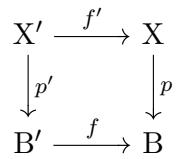
\includegraphics[keepaspectratio]{images/part001_dd3067cf.jpg}}

(E, II, p. 14). 于是我们说“考虑方块图 (1)”，或简单地说“方块 (1)”，以代替说“考虑连续映射的四元组 \(f,f^{\prime},p,p^{\prime}\) ”。称方块 (1) 为交换的，如果等式

\[
f \circ p ^ {\prime} = p \circ f ^ {\prime}
\]

成立。在这情形下，常给 B′、X 与 X′ 分别装备由映射 f、p 与 \(f \circ p' = p \circ f'\) 所定义的 B-空间结构；此时映射 \(p'\) 与 \(f'\) 是 B-态射。

定义 4. --- 我们称方块 (1) 为拓扑空间的笛卡尔方块（或简单地称它是笛卡尔的），如果它是交换的，并且对每个拓扑空间 Y 和每对连续映射 u: Y → B' 与 v: Y → X（满足 f ∘ u = p ∘ v），存在唯一的连续映射 w: Y → X'，满足 p' ∘ w = u 且 f' ∘ w = v。

为使方块 (1) 是笛卡尔的，必须且只需方块

(1')

\pandocbounded{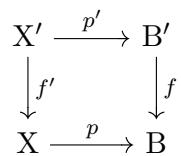
\includegraphics[keepaspectratio]{images/part001_f0fdde30.jpg}}

是笛卡尔的。

命题 1. --- 为使方块 (1) 是笛卡尔的，必须且只需它是交换的，并且对每个 B-空间 Y 和每对 B-态射 \(u\colon Y \to B'\) 、\(v\colon Y \to X\) ，存在唯一的 B-态射 \(w\colon Y \to X'\) ，使得 \(p' \circ w = u\) 且 \(f' \circ w = v\) 。

设方块 (1) 是笛卡尔的。设 Y 为一个 B-空间，\(u: Y \to B'\) 与 \(v: Y \to X\) 为 B-态射。映射 \(f \circ u\) 与 \(p \circ v\) 都等于 B-空间 Y 的投影；于是满足 \(p' \circ w = u\) 与 \(f' \circ w = v\) 的唯一连续映射 w 是一个 B-态射。这就证明了条件的必要性。

反之，设此条件成立。设 Y 为一个拓扑空间，\(u \colon \mathrm{Y} \to \mathrm{B}'\) 与 \(v \colon \mathrm{Y} \to \mathrm{X}\) 为满足 \(f \circ u = p \circ v\) 的连续映射。当 Y 装备上由 \(f \circ u\) 定义的 B-空间结构时，\(u\) 与 \(v\) 是 B-态射。每个连续映射 \(w \colon \mathrm{Y} \to \mathrm{X}'\) ，只要满足 \(p' \circ w = u\) 与 \(f' \circ w = v\) ，就是一个 B-态射，所以这样的映射恰好存在一个。

命题 2. --- 设 B、B' 与 X 为拓扑空间，p: X → B、f: B' → B 为连续映射。

\begin{enumerate}
\def\labelenumi{\alph{enumi})}
\tightlist
\item
  方块
\end{enumerate}

\[
\begin{array}{c} \mathrm{B} ^ {\prime} \times_ {\mathrm{B}} \mathrm{X} \xrightarrow {\mathrm{pr} _ {2}} \mathrm{X} \\ \Biggl \downarrow \mathrm{pr} _ {1} \\ \mathrm{B} ^ {\prime} \xrightarrow {f} \mathrm{B} \end{array}\tag{2}
\]

是一个笛卡尔方块。

\begin{enumerate}
\def\labelenumi{\alph{enumi})}
\setcounter{enumi}{1}
\tightlist
\item
  对每个交换方块
\end{enumerate}

\[
\begin{array}{c} \mathrm {X^ {\prime}} \xrightarrow {f ^ {\prime}} \mathrm{X} \\ \Big \downarrow_ {p ^ {\prime}} \\ \mathrm {B^ {\prime}} \xrightarrow {f} \mathrm{B} \end{array}\tag{3}
\]

存在唯一的连续映射 \(h: X' \to B' \times_{B} X\) ，使得 \(pr_{1} \circ h = p'\) 且 \(pr_{2} \circ h = f'\) 。

\begin{enumerate}
\def\labelenumi{\alph{enumi})}
\setcounter{enumi}{2}
\tightlist
\item
  交换方块 (3) 是笛卡尔的，当且仅当 h 是一个同胚。
\end{enumerate}

断言 \(a\) ) 由命题 1 以及 B-空间的范畴中两个 B-空间的积的泛性质 (I, p. 3) 得出。断言 \(b\) ) 由它得出。

若方块 (3) 是笛卡尔的，则存在唯一的连续映射 \(h'\colon B'\times_{B}X\to X'\) ，使得 \(f'\circ h' = pr_{2}\) 且 \(p'\circ h' = pr_{1}\) 。我们有 \(f'\circ h'\circ h = f'\) 与 \(p'\circ h'\circ h = p'\) ，由于方块 (3) 是笛卡尔的，从而 \(h'\circ h = Id_{X'}\) 。我们有 \(pr_{1}\circ h\circ h' = pr_{1}\) 与 \(pr_{2}\circ h\circ h' = pr_{2}\) ，由于方块 (2) 是笛卡尔的，从而 \(h\circ h' = Id_{B'\times_{B}X}\) 。这就证明了 h 是一个同胚。

反之，设 h 是一个同胚；由于方块 (2) 是笛卡尔的，方块 (3) 也是笛卡尔的。

映射 \(h \colon \mathrm{X}' \to \mathrm{B}' \times_{\mathrm{B}} \mathrm{X}\) ——其存在性与唯一性由前一命题的 \(b)\) 款所断言——将称为典型的：它就是在 I, p. 3 中记作 \((p', f')\) 的映射。

命题 3. --- 设

\[
\begin{array}{c} \mathrm {X^ {\prime}} \xrightarrow {f ^ {\prime}} \mathrm{X} \\ \Big \downarrow_ {p ^ {\prime}} \\ \mathrm {B^ {\prime}} \xrightarrow {f} \mathrm{B} \end{array}
\]

为一个笛卡尔方块。对 \(p'\) 的任一连续截面 s，映射 \(f'\circ s\) 是 f 到 X 中的连续提升。映射 \(s\mapsto f'\circ s\) 是从 \(\mathcal{C}_{\mathrm{B}'}(\mathrm{B}';\mathrm{X}')\) 到 \(\mathcal{C}_{\mathrm{B}}(\mathrm{B}';\mathrm{X})\) 上的一个双射。

若 \(s \colon B' \to X'\) 是 \(p'\) 的一个连续截面，我们有 \(p \circ f' \circ s = f \circ p' \circ s = f\) ，这就证明 \(f' \circ s\) 是 \(f\) 到 X 中的连续提升，即从 \(B'\) 到 X 中的一个 B-态射。反之，设 \(g \colon B' \to X\) 是一个 B-态射。我们有 \(f \circ \mathrm{Id}_{\mathrm{B}'} = p \circ g\) ；于是由笛卡尔方块的定义，存在唯一的连续映射 \(s \colon B' \to X'\) ，使得 \(p' \circ s = \mathrm{Id}_{\mathrm{B}'}\) 且 \(f' \circ s = g\) ，命题得证。

